% ==============================================================================
% DIDAKTISCHE ENTWICKLER-RICHTLINIEN FÜR KAPITEL 1 (PYTHON-SYNTAX & CONTAINER)
% ==============================================================================
% Dieses Kapitel dient als praktisches Nachschlagewerk zum Schreiben von Code in
% der Prüfung. Zukünftige KIs und Entwickler müssen folgende Konventionen einhalten:
%
% 1. VARIABLE BENENNUNG:
%    - Keine abstrakten Namen wie 'a', 'b', 'x', 'y' (ausser bei kurzen Indizes).
%    - Einheitliche Container-Variablen: 'lst' für Liste, 'tup' für Tupel,
%      'set_a'/'set_b' für Sets (nie 's', um Verwechslung mit Strings zu vermeiden),
%      'mein_dict' oder konkrete Beispiele (wie 'alter') für Dictionaries.
%    - Echte Use-Cases: Mappings anschaulich benennen, z. B. 'alter = {"Alice": 20}'
%      oder 'namen'/'alter' bei zip, um den Nutzen der Struktur sofort zu verdeutlichen.
%    - Verschachtelte Comprehensions nutzen 'aussen' und 'innen' als Loop-Variablen bei
%      Verschachtelungen, um die Evaluierungsreihenfolge klarzumachen.
%
% 2. KOMMENTAR-STRUKTUR & LAYOUT:
%    - Einfache, noob-freundliche Sprache. Jargon wie "In-Place" oder "Shallow Copy"
%      im Kommentar durch beschreibende Sätze ersetzen (z. B. "ändert Liste direkt",
%      "erzeugt Kopie, Änderungen betreffen das Original nicht").
%    - Keine Angabe von asymptotischen Laufzeiten (O-Notation) oder Exception-Klassen
%      (wie ValueError, KeyError) - dieses Kapitel fokussiert rein auf Syntaxpraxis.
%    - PLATZIERUNG & SPACING: Kommentare gehören rechts neben den Code, niemals in
%      eine eigene Zeile darüber (ausser bei sehr langen Codezeilen). Auf starre
%      tabellarische Ausrichtung (gleiche Spalte für '#') verzichten. Stattdessen nur
%      1-2 Leerzeichen Abstand vor '#' nutzen, um Zeilenumbrüche und damit unnötigen
%      vertikalen Platzverbrauch im Spaltenlayout zu verhindern.
%
% 3. LATEX-BESONDERHEITEN:
%    - In den optionalen Kommentar-Argumenten [comment] von \CodeLine darf NIEMALS
%      ein rohes '_' (Unterstrich) oder '&' (Kaufmanns-Und) verwendet werden.
%      Der Unterstrich erzeugt einen Mathe-Subscript-Fehler, das '&' einen Alignment-
%      Tab-Fehler. Nutzen Sie stattdessen 'und' oder schreiben Sie Begriffe gross
%      (z. B. 'Set A' statt 'set_a').
% ==============================================================================

\section{Python-Syntax \& Container}\label{sec:01-python-syntax-übersicht}

\begin{chapterindex}
\ZSFChapterIndexGroup{sec:01-grundlagen}{Grundlagen \& Schleifen-Idiome}
\ZSFChapterIndexEntry{sec:01-datentypen}{Datentypen \& Typprüfung}
\ZSFChapterIndexEntry{sec:01-operatoren}{Operatoren \& Logik}
\ZSFChapterIndexEntry{sec:01-kontrollstrukturen}{Schleifen-Kontrolle}
\ZSFChapterIndexEntry{sec:01-funktionen}{Funktionen \& Standardwerte}
\ZSFChapterIndexGroup{sec:01-container-überblick}{Container-Überblick}
\ZSFChapterIndexEntry{sec:01-python-container}{Container-Typen im Vergleich}
\ZSFChapterIndexGroup{sec:01-sequenzen}{Sequenzen: Listen \& Tupel}
\ZSFChapterIndexEntry{sec:01-operationen-auf-containern}{Grundoperationen für Sequenzen}
\ZSFChapterIndexEntry{sec:01-sequenzen-geordnete-container}{Veränderbarkeit \& Unpacking}
\ZSFChapterIndexEntry{sec:01-slicing-details}{Slicing-Tricks}
\ZSFChapterIndexEntry{sec:01-allgemeine-sequenz-operationen}{Sequenz-Operationen}
\ZSFChapterIndexEntry{sec:01-häufige-listen-operationen}{Listen-Manipulation}
\ZSFChapterIndexEntry{sec:01-sortieren-mit-keys}{Sortieren \& Extremwerte}
\ZSFChapterIndexEntry{sec:01-list-comprehension}{Comprehensions: List, Dictionary, Set}
\ZSFChapterIndexEntry{sec:01-grid-init}{Grids: Initialisierung \& Kopieren}
\ZSFChapterIndexGroup{sec:01-sets-und-dictionaries}{Assoziative Container (Sets \& Dictionaries)}
\ZSFChapterIndexEntry{sec:01-collections-ungeordnete-container}{Set und Dictionary im Vergleich}
\ZSFChapterIndexEntry{sec:01-set-operationen}{Mengen-Operationen (Sets)}
\ZSFChapterIndexEntry{sec:01-dictionary-operationen}{Dictionary-Zugriff \& Updates}
\ZSFChapterIndexEntry{sec:01-iteration-über-ein-dictionary}{Dictionary-Iteration}
\ZSFChapterIndexGroup{sec:01-container-erzeugen}{Container erzeugen \& kombinieren}
\ZSFChapterIndexEntry{sec:01-list-comprehension}{Comprehensions: List, Dictionary, Set}
\ZSFChapterIndexGroup{sec:01-zip}{Gemeinsame Iteration mit \texttt{zip}}
\ZSFChapterIndexEntry{sec:01-zip-pairs}{Element-Paarung}
\ZSFChapterIndexGroup{sec:01-strings}{Strings}
\ZSFChapterIndexEntry{sec:01-string-methoden-referenz}{String-Manipulation}
\end{chapterindex}

% -----------------------------
\ZSFmanualColumnBreak
\subsection{Grundlagen \& Schleifen-Idiome}\label{sec:01-grundlagen}
\subsubsection{Datentypen \& Typprüfung}\label{sec:01-datentypen}
\begin{contentbox}
\CodeLine{zahl = 5}[int]\\
\CodeLine{komma = 3.14}[float]\\
\CodeLine{text = "hello"}[string]\\
\CodeLine{logisch = True}[boolean]\\
\CodeLine{leerr = None}[Nullwert / leerer Wert (Prüfung mit: x is None)]\\
\CodeLine{leerr is None}[True (Identitaets-Vergleich; bevorzugen fuer None)]\\
\CodeLine{bool(0), bool(""), bool([]), bool(None)}[alle False (leere Container / Nullwerte)]\\
\CodeLine{isinstance(zahl, int)}[True (prüft auch Unterklassen; bevorzugen!)]\\
\CodeLine{str(5), int("5"), float("3.14")}[Typ-Konvertierung (zu String, Integer, Float)]\\
String-Methoden \ZSFarrowref{sec:01-string-methoden-referenz}
\end{contentbox}

% -----------------------------
\subsubsection{Operatoren \& Logik}\label{sec:01-operatoren}
\begin{contentbox}
\CodeLine{5 / 2, 5 // 2, 5 \% 2}[2.5 (Float-Div), 2 (Ganzzahl-Div), 1 (Modulo)]\\
\CodeLine{2 ** 3, abs(-5), round(3.141, 2)}[8 (Potenz), 5 (Absolutwert), 3.14 (Runden)]\\
\CodeLine{quotient, rest = divmod(17, 5)}[quotient=3, rest=2 (Ganzzahl-Division und Rest zusammen)]\\
\CodeLine{chr(65), ord("A")}[Zahl zu Zeichen, Zeichen zu Zahl]\\
\CodeLine{a and b, a or b, not a}[Logische Operatoren (nicht \&\&, ||, !)]\\
\CodeLine{1 < x < 10}[Verketteter Vergleich (True, wenn x zwischen 1 und 10)]\\
\CodeLine{x == y, x is y}[Wertgleichheit vs. Speicher-Identitaet]
\end{contentbox}

% -----------------------------
\subsubsection{Schleifen-Kontrolle}\label{sec:01-kontrollstrukturen}
\ZSFindex{enumerate}
\begin{codebox}[Iteration (\texttt{for}, \texttt{enumerate}, \texttt{while})]
\begin{lstlisting}[style=CodeExpert]
# range(start, stop, step): stop exklusiv!
for i in range(0, 10, 2):   # 0, 2, 4, 6, 8 (Schrittweite 2)
    print(i)

for i in range(5, 1, -1):   # 5, 4, 3, 2 (rueckwaerts)
    print(i)

for zeichen in "abc":  # über jedes Zeichen einzeln iterieren
    print(zeichen)

# enumerate() liefert Paare (Index, Element) -> idx = Index, wert = Element
for idx, wert in enumerate(["a", "b"]):
    print(idx, wert)

# while wiederholt, solange eine beliebige Bedingung True ist
while N > 0:
    ziffer = N % 10   # letzte Ziffer holen
    N //= 10          # letzte Ziffer entfernen

# items() liefert Paare (Schlüssel, Wert) -> name = Key, alter = Value
for name, alter in {"Alice": 20, "Bob": 22}.items():
    print(name, alter)
\end{lstlisting}
Dictionary-Iteration \ZSFarrowref{sec:01-iteration-über-ein-dictionary}\enspace
\texttt{zip} \ZSFarrowref{sec:01-zip}
\end{codebox}

\begin{codebox}[Schleifensteuerung (\texttt{break} vs. \texttt{continue})]
\begin{lstlisting}[style=CodeExpert]
# continue: Durchlauf überspringen | break: Schleife beenden
for i in range(1, 6):
    if i == 2:
        continue  # i=2 überspringen (Rest im Durchlauf auslassen)
    if i == 4:
        break     # Schleife bei i=4 sofort verlassen
    print(i)      # Ausgabe: 1, 3
\end{lstlisting}
\texttt{break} und \texttt{continue} wirken immer NUR auf die am tiefsten verschachtelte (innerste) Schleife (\texttt{for}, \texttt{while}), in der sie sich direkt befinden. Die äussere Schleife läuft danach ganz normal weiter!
\end{codebox}

% -----------------------------
\subsubsection{Funktionen \& Standardwerte}\label{sec:01-funktionen}
\begin{codebox}
\begin{lstlisting}[style=CodeExpert]
# Funktionsdefinition
def summe(x, y):
    return x + y

# Aufruf mit Argumenten
summe(2, 3)

def gruss(name="Gast"):    # Standardwert (wird genutzt, wenn kein Wert übergeben wird)
    return "Hallo " + name

\end{lstlisting}
Key-Sortierung \ZSFarrowref{sec:01-sortieren-mit-keys}
\end{codebox}

% -----------------------------
\subsection{Container-Überblick}\label{sec:01-container-überblick}
\ZSFindex{Liste}
\ZSFindex{Tupel}
\subsubsection{Container-Typen im Vergleich}\label{sec:01-python-container}
\begin{codebox}
\begin{lstlisting}[style=CodeExpert]
# Sequenzen: geordnet, Zugriff über Index
lst = [1, 2, 2]                  # veränderbar, Duplikate erlaubt
tup = (1, 2, 2)                  # unveränderbar, Duplikate erlaubt
zahlen = range(1, 4)             # unveränderbare Folge von Ganzzahlen
text = "Hallo"                   # unveränderbare Folge von Zeichen

# Kollektionen: Zugriff nicht über Position
set_a = {1, 2, 3}                # veränderbar, keine Duplikate
dict_alter = {"Alice": 20}       # veränderbar, eindeutige Schlüssel
\end{lstlisting}
Listen \& Tupel \ZSFarrowref{sec:01-operationen-auf-containern}\enspace
Sets \ZSFarrowref{sec:01-set-operationen}\enspace
Dictionaries \ZSFarrowref{sec:01-dictionary-operationen}\enspace
Strings \ZSFarrowref{sec:01-string-methoden-referenz}
\end{codebox}

\begin{contentbox}[Taxonomie]
\begin{center}
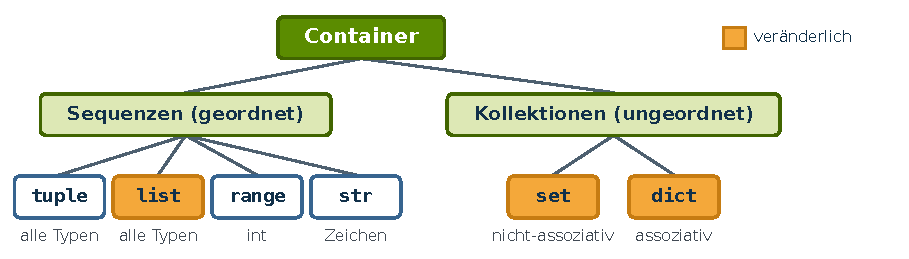
\includegraphics[width=\columnwidth]{Images/python-container-taxonomy-sequence-collection.pdf}
\end{center}
\end{contentbox}

% -----------------------------
\subsection{Sequenzen: Listen \& Tupel}\label{sec:01-sequenzen}
\subsubsection{Grundoperationen für Sequenzen}\label{sec:01-operationen-auf-containern}
\begin{codebox}[Elemente suchen \& prüfen]
\begin{lstlisting}[style=CodeExpert]
len(lst)                            # gibt die Anzahl der Elemente zurück
wert in daten                       # prüft direkt, ob der Wert enthalten ist
wert not in daten                   # prüft direkt, ob der Wert fehlt
daten.count(wert)                   # zählt den Wert ohne eigene Schleife
daten.index(wert)                   # Position des ersten Treffers

# True, wenn die Bedingung für mindestens ein Element gilt
any([bedingung(element) for element in daten])
# True, wenn die Bedingung für alle Elemente gilt
all([bedingung(element) for element in daten])
\end{lstlisting}
Listen-Methoden \ZSFarrowref{sec:01-häufige-listen-operationen}\enspace
Comprehensions \ZSFarrowref{sec:01-list-comprehension}
\end{codebox}

\begin{codebox}[Zugriff, Mathe \& Sortierung]
\begin{lstlisting}[style=CodeExpert]
lst[0], tup[0]                      # Indexzugriff
lst[1:3]                            # Slicing
lst[start:stop:step]                # Slicing: Ausschnitt holen (start inkl., stop exkl.)
max(lst, default=0), min(lst)      # Maximum / Minimum (default sichert gegen leere Liste ab)
sum(lst)                            # Summe aller Elemente
list("abc")                         # erzeugt die Liste ['a', 'b', 'c']
tuple(lst)                          # in tuple umwandeln
sorted(lst)                         # erzeugt neue sortierte Liste (Original bleibt gleich)
\end{lstlisting}
Slicing \ZSFarrowref{sec:01-slicing-details}
\end{codebox}

% -----------------------------
\subsubsection{Veränderbarkeit \& Unpacking}\label{sec:01-sequenzen-geordnete-container}
\begin{codebox}
\begin{lstlisting}[style=CodeExpert]
# veränderbare Sequenz
lst = [10, 20, 30]
# unveränderbare Sequenz
tup = (10, 20, 30)
# unveränderbare Zeichenkette
s = "abc"
lst[0], tup[1], s[2]         # Indexzugriff
lst[1:]                      # Slicing

# Sequenz-Unpacking
tup_3 = (1, 2, 3)
a, b, c = tup_3              # a=1, b=2, c=3 (Entpacken)
a, b = b, a                # Wertetausch ohne Hilfsvariable

# Unpacking mit * (Rest-Elemente sammeln)
first, *rest = [1, 2, 3, 4] # first=1, rest=[2, 3, 4]
*init, last = [1, 2, 3, 4]  # init=[1, 2, 3], last=4

\end{lstlisting}
Slicing \ZSFarrowref{sec:01-slicing-details}
\end{codebox}

% -----------------------------
\subsubsection{Slicing-Tricks}\label{sec:01-slicing-details}
\ZSFindex{Slicing}
\begin{codebox}
\begin{lstlisting}[style=CodeExpert]
lst = [10,20,30,40,50] # lst[start:stop:step]
# start inklusive, stop exklusiv, Standardschritt=1
lst[1:4] # [20,30,40] (von Index 1 bis 3) | lst[:]=Kopie
lst[-1] # 50 (letztes Element) | lst[-2:] = die letzten beiden
lst[::2] # [10,30,50] | lst[::-1] = umgedrehte Kopie
lst[4:1:-1] # [50,40,30] (rückwärts von Index 4 bis 2)
kopie = lst[:] # Kopie der Liste (Änderung an kopie ändert lst nicht)
lst[1:3] = [0,0,0] # ersetzt Bereich durch 3 Werte (Liste wird länger!)
lst[1:3] = [] # löscht den Bereich aus der Liste
list(reversed(lst)) # umgedrehte Kopie; reversed(lst) zum Rückwärts-Iterieren
"python"[::-1] # erzeugt umgedrehten neuen String
\end{lstlisting}
String-Methoden \ZSFarrowref{sec:01-string-methoden-referenz}
\end{codebox}

% -----------------------------
\subsubsection{Sequenz-Operationen}\label{sec:01-allgemeine-sequenz-operationen}
\begin{codebox}
\begin{lstlisting}[style=CodeExpert]
[1, 2] + [3, 4] # Verkettung: verbindet zu [1, 2, 3, 4]
[1] * 3         # Wiederholung: erzeugt [1, 1, 1]
# Listen automatisch aus Variablen erzeugen
lst = []                    # leere Liste zum spaeteren Befuellen
lst = [startwert] * n       # erzeugt n gleiche Startwerte
lst = list(range(n))        # erzeugt Werte von 0 bis n-1 ([0, 1, ..., n-1])
lst = list(range(1, 10, 2)) # [1, 3, 5, 7, 9] (start, stop, step)
lst = [1, 2, 3]
# Kopieren vs. Aliasing
b = lst          # Alias: Aenderungen an b betreffen auch lst!
b = lst[:]       # flache Kopie (Aenderung an b betrifft lst nicht)

# ueber Sequenz iterieren
for element in lst:
    print(element)
\end{lstlisting}
Aus vorhandenen Daten erzeugen oder filtern: Comprehensions \ZSFarrowref{sec:01-list-comprehension}
\end{codebox}

% -----------------------------
\subsubsection{Listen-Manipulation}\label{sec:01-häufige-listen-operationen}
\ZSFindex[sortieren]{Sortieren}
\begin{contentbox}
\CodeLine{lst.append(4)}[ans Ende anfügen]\\
\CodeLine{lst.extend([5, 6])}[fügt Elemente einer Liste einzeln hinten an]\\
\CodeLine{lst.insert(1, 99)}[fügt 99 an Index 1 ein (verschiebt den Rest nach hinten)]\\
\CodeLine{lst.remove(1)}[sucht und löscht die erste 1 (Fehler falls nicht da)]\\
\CodeLine{lst.pop()}[löscht und gibt letztes Element zurück (pop(i) löscht an Index i)]\\
\CodeLine{del lst[0]}[per Index löschen]\\
\CodeLine{kopie = lst.copy()}[flache Kopie der Liste]\\
\CodeLine{lst.clear()}[alle Elemente löschen]\\
\CodeLine{lst.sort()}[sortiert direkt (Achtung: gibt None zurück!) \ZSFref{sec:04-algorithmen}]\\
\CodeLine{lst.reverse()}[dreht Reihenfolge direkt um (ändert Original)]
\end{contentbox}

\subsubsection{Sortieren \& Extremwerte}\label{sec:01-sortieren-mit-keys}
\begin{codebox}
\begin{lstlisting}[style=CodeExpert]
# sorted() erzeugt neue sortierte Liste, Original bleibt gleich
sorted([-3, 1, -2], key=abs)  # [1, -2, -3] (nach Absolutwert)
sorted(lst_namen, key=len)    # sortiert nach Wortlaenge
sorted(lst_namen, key=lambda x: (len(x), x)) # Tupel-Sort: erst Laenge, dann alphabetisch (lexikographisch)
# max() / min() unterstuetzen auch key= und default=
max(lst_namen, key=len, default="") # laengstes Wort (default sichert leere Liste ab)
\end{lstlisting}
\end{codebox}

% -----------------------------
\subsubsection{Grids: Initialisierung \& Kopieren}\label{sec:01-grid-init}
\begin{codebox}[2D-Grid anlegen \& Deepcopy]
\begin{lstlisting}[style=CodeExpert]
# 2D-Grid richtig initialisieren (vermeidet Referenz-Sharing)
grid = [[0] * n for _ in range(m)] # m unabhaengige Zeilen
# [[0]*n]*m erzeugt nur m Referenzen auf dieselbe Zeile!

\end{lstlisting}
Comprehensions \ZSFarrowref{sec:01-list-comprehension}
\end{codebox}

% -----------------------------
\subsection{Assoziative Container (Sets \& Dictionaries)}\label{sec:01-sets-und-dictionaries}
\ZSFindex{Set}
\ZSFindex{Dictionary}
\subsubsection{Set und Dictionary im Vergleich}\label{sec:01-collections-ungeordnete-container}
\begin{codebox}
\begin{lstlisting}[style=CodeExpert]
# set: ungeordnet, keine Duplikate. Schnelle Suche mit 'in'
set_a = {1, 2, 3}
set_a = set()                # leeres Set; {} waere ein leeres Dict
set_a = set(lst)             # aus Daten; entfernt Duplikate

alter = {"Alice": 20, "Bob": 22}       # dict: Schlüssel-Wert
# sets sind schnell für Enthaltensein-Prüfung,
# kein Indexzugriff
2 in set_a                    # Enthaltensein prüfen
len(set_a)                    # Anzahl Elemente
\end{lstlisting}
Automatisch erzeugen oder filtern: Comprehensions \ZSFarrowref{sec:01-list-comprehension}
\end{codebox}

% -----------------------------
\subsubsection{Mengen-Operationen (Sets)}\label{sec:01-set-operationen}
\begin{contentbox}
\texttt{set\_a = \{1, 2, 3\}},\ \texttt{set\_b = \{3, 4, 5\}}\\
\CodeLine{set_a | set_b}[Vereinigung: alle Elemente aus Set A und Set B]\\
\CodeLine{set_a & set_b}[Schnittmenge: nur Elemente, die in beiden sind]\\
\CodeLine{set_a - set_b}[Differenz: Elemente in Set A, die nicht in Set B sind]\\
\CodeLine{set_a ^ set_b}[Elemente, die genau in einem Set sind]\\
\CodeLine{set_a.add(6)}[Element hinzufügen]\\
\CodeLine{set_a.remove(1)}[löscht 1 aus Set (Fehler falls nicht da)]\\
\CodeLine{set_a.discard(1)}[löscht 1 sicher; kein Fehler falls nicht da]\\
\CodeLine{set_a.update([6, 7])}[fügt alle Elemente aus den Daten hinzu]\\
\CodeLine{set_a.isdisjoint(set_b)}[True, wenn beide Sets keine gemeinsamen Elemente haben]\\
\CodeLine{x in set_a}[True, wenn x in Set A enthalten]
\end{contentbox}

% -----------------------------
\subsubsection{Dictionary-Zugriff \& Updates}\label{sec:01-dictionary-operationen}
\begin{contentbox}
\CodeLine{daten = dict()}[leeres Dictionary zum schrittweisen Befüllen]\\
\CodeLine{daten = dict(paare)}[erzeugt Dictionary aus Schlüssel-Wert-Paaren]\\
\CodeLine{daten = dict(zip(keys, werte))}[verbindet zwei Container zu Schlüssel und Wert]\\
\CodeLine{daten = dict.fromkeys(namen, 0)}[alle Namen als Schlüssel mit Startwert 0]\\
Automatisch aus Daten erzeugen: Comprehensions \ZSFarrowref{sec:01-list-comprehension}\\
\texttt{alter = \{"Alice": 20, "Bob": 22\}}\\
\CodeLine{alter["Charlie"] = 25}[Schlüssel hinzufügen / aktualisieren]\\
\CodeLine{alter.get("Alice", 0)}[holt Wert für "Alice", sonst 0]\\
\CodeLine{daten[key] = daten.get(key, 0) + wert}[fehlender Schlüssel startet bei 0, vorhandener Wert wird erhöht]\\
\CodeLine{alter.pop("Bob", None)}[löscht sicher: gibt None zurück, falls Key fehlt (kein Fehler)]\\
\CodeLine{del alter["Bob"]}[löscht Schlüssel "Bob" (Fehler falls nicht da)]\\
\CodeLine{"Alice" in alter}[Enthaltensein prüfen]\\
\CodeLine{list(alter.keys())}[Liste der Schlüssel (Namen)]\\
\CodeLine{list(alter.values())}[Liste der Werte (Alter)]\\
\CodeLine{list(alter.items())}[Liste der (Schlüssel, Wert)-Paare]\\
\CodeLine{max(alter, key=alter.get)}[liefert Schluessel mit groesstem Wert (Charlie)]\\
\CodeLine{{**alter, **neu}}[erzeugt zusammengefuegte Kopie (Mergen)]
\end{contentbox}

% -----------------------------
\subsubsection{Dictionary-Iteration}\label{sec:01-iteration-über-ein-dictionary}
\begin{codebox}
\begin{lstlisting}[style=CodeExpert]
alter = {"Alice": 20, "Bob": 22}

for name in alter:                # Achtung: Iteriert standardmässig NUR über Schlüssel!
    print(name)

for jahre in alter.values():       # Werte
    print(jahre)

for name, jahre in alter.items():     # Schlüssel und Werte
    print(name, jahre)

# mit Index
for idx, (name, jahre) in enumerate(alter.items()):
    print(idx, name, jahre)
\end{lstlisting}
Schleifen \& \texttt{enumerate} \ZSFarrowref{sec:01-kontrollstrukturen}\enspace
\texttt{zip} \ZSFarrowref{sec:01-zip}
\end{codebox}

% -----------------------------
\subsection{Container erzeugen \& kombinieren}\label{sec:01-container-erzeugen}
\subsubsection{Comprehensions: List, Dictionary, Set}\label{sec:01-list-comprehension}
\ZSFindex{List Comprehension}
\begin{codebox}
\begin{lstlisting}[style=CodeExpert]
# Form: Ausdruck for Element in Daten, optional mit if Bedingung
namen = ["Ada", "Bob", "Ada Lovelace"]

# List: Elemente verarbeiten oder filtern
[name.upper() for name in namen]        # neue Liste, Namen gross
[name for name in namen if len(name) > 3] # nur passende Namen
# Ternary Operator: if-else steht vor dem for
[zahl if zahl > 0 else 0 for zahl in [-1, 2, -3]]
# verschachtelte Schleifen: links steht die aeussere, rechts die innere
[(aussen, innen) for aussen in [1,2] for innen in [3,4]]

# Dict: Schluessel und Werte aus vorhandenen Daten erzeugen
{name: 0 for name in namen}             # gleicher Startwert je Name
{name: len(name) for name in namen}     # Wert aus Element berechnen

# Set: verarbeiten; gleiche Ergebnisse nur einmal speichern
{name.lower() for name in namen}        # erzeugt Set ohne Duplikate

# Container mit * zusammensetzen
kombiniert = [*liste_a, *liste_b]       # verbindet zwei Listen
alle_werte = {*set_a, *set_b}           # verbindet Sets, Duplikate nur einmal
\end{lstlisting}
Listen-Methoden \ZSFarrowref{sec:01-häufige-listen-operationen}\enspace
Sets \ZSFarrowref{sec:01-set-operationen}\enspace
Dictionaries \ZSFarrowref{sec:01-dictionary-operationen}
\end{codebox}

% -----------------------------
\subsection{Gemeinsame Iteration mit \texttt{zip}}\label{sec:01-zip}
\subsubsection{Element-Paarung}\label{sec:01-zip-pairs}
\ZSFindex{zip}
\begin{codebox}
\begin{lstlisting}[style=CodeExpert]
namen = ["Alice", "Bob", "Charlie"]
alter = [20, 22, 25]
paare = list(zip(namen, alter)) # gleiche Positionen zu Paaren verbinden
print(paare) # [("Alice", 20), ("Bob", 22), ("Charlie", 25)]
for name, jahre in zip(namen, alter): # auch in for-Schleifen verwendbar
    print(name, jahre)

# Gemeinsame Werte: Reihenfolge von namen bleibt erhalten
andere_namen = ["Bob", "Charlie", "Dana"]
gemeinsam = [name for name in namen if name in andere_namen]
# ["Bob", "Charlie"]

daten = ["A", "B", "C"]
# Nachbarn vergleichen: jedes Element mit seinem direkten Nachfolger
for vorher, aktuell in zip(daten, daten[1:]):
    print(vorher, aktuell) # ("A", "B"), dann ("B", "C")

# Drei aufeinanderfolgende Werte gleichzeitig prüfen
for links, mitte, rechts in zip(daten, daten[1:], daten[2:]):
    print(links, mitte, rechts)
\end{lstlisting}
Dictionary aus Paaren \ZSFarrowref{sec:01-dictionary-operationen}
\end{codebox}

% -----------------------------
\ZSFmanualColumnBreak
\subsection{Strings}\label{sec:01-strings}
\subsubsection{String-Manipulation}\label{sec:01-string-methoden-referenz}
\ZSFindex{String}
\begin{codebox}
\begin{lstlisting}[style=CodeExpert]
text = "  Hello World  "
text.strip()                  # entfernt Leerzeichen (auch \n, \t) an Enden | strip("!?") entfernt custom Zeichen an Enden
text.lower(), text.upper()    # alles klein / gross schreiben
text.startswith("He")         # True (prueft Praefix)
text.endswith("ld")           # True (prueft Suffix)
text.find("lo")               # Index des 1. Treffers (von links), -1 falls nicht da
text.rfind("l")               # Index des 1. Treffers von rechts (Zeitspar-Abkuerzung!), -1 falls nicht da
text.count("l")               # zaehlt Vorkommen des Teilstrings
text.replace("World", "Python") # ersetzt ALLE Vorkommen im gesamten String (replace("a", "") loescht)

# Aufteilen und Verbinden
"Hello" + " " + "World"       # "Hello World" (zusammenfuegen / verketten mit +)
text.split()                  # trennt an Leerzeichen (entfernt auch doppelte)
text.split("o")               # trennt an custom Zeichen
"-".join(["a", "b"])          # verbindet Liste zu String -> "a-b"
"".join(list("abc"))          # baut String aus Zeichenliste

# Pruefung und Umwandlung
"123".isdigit()               # True (nur Ziffern?) | isalpha() (nur Buchstaben?) | isalnum() (beides?) | islower()/isupper()
"lo" in "hello"               # True (Teilstring-Suche / Enthaltensein)
list("abc")                   # ['a', 'b', 'c'] (in Liste umwandeln)
\end{lstlisting}
Slicing \ZSFarrowref{sec:01-slicing-details}
\end{codebox}
